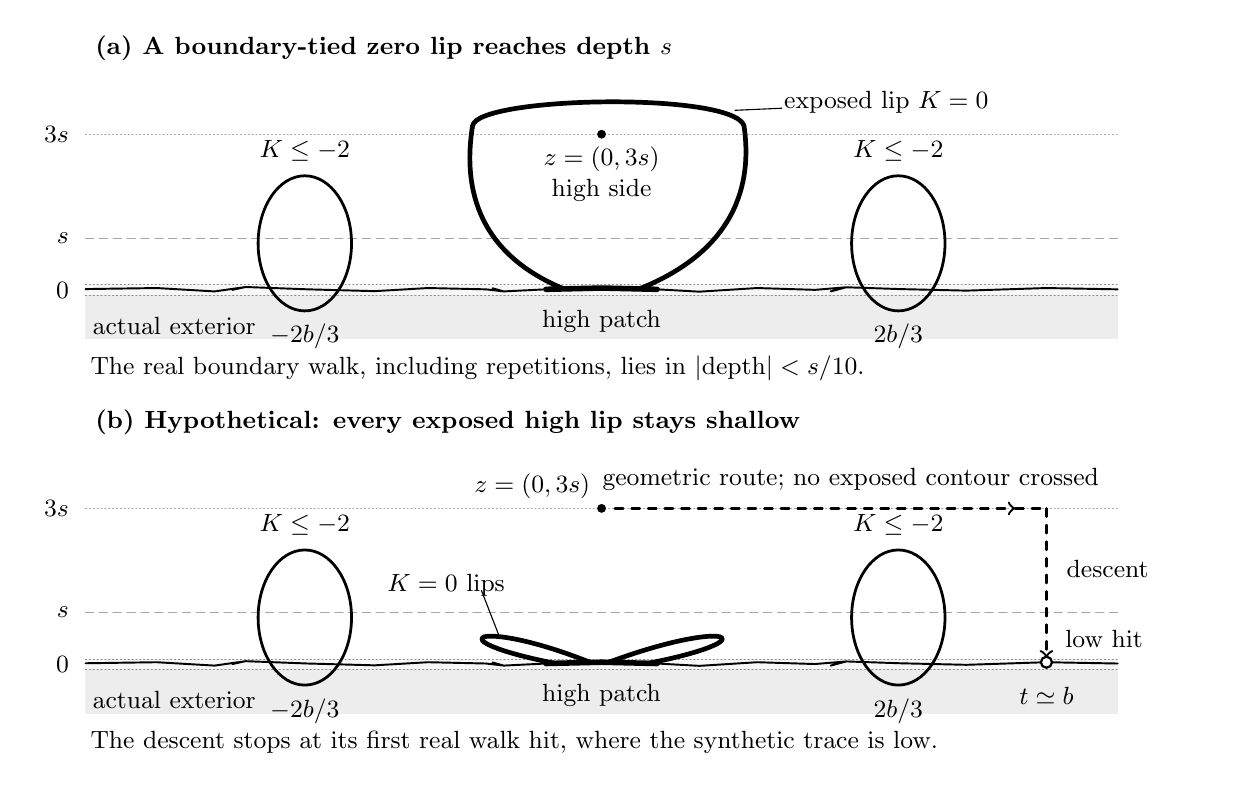
\begin{tikzpicture}[x=5.65cm,y=0.66cm,
  font=\fontsize{9}{11}\selectfont,line cap=round,line join=round]
\path[use as bounding box] (-1.29,-9.0) rectangle (1.36,5.05);
\foreach \panelshift in {0,-7.2} {
  \begin{scope}[shift={(0,\panelshift)}]
    \fill[black!7] (-1.16,-0.95) rectangle (1.16,-0.1);
    \fill[black!3] (-1.16,-0.1) rectangle (1.16,0.1);
    \draw[black!45,densely dotted] (-1.16,-0.1) -- (1.16,-0.1);
    \draw[black!45,densely dotted] (-1.16,0.1) -- (1.16,0.1);
    \draw[black!35,densely dashed] (-1.16,1) -- (1.16,1);
    \draw[black!35,densely dotted] (-1.16,3) -- (1.16,3);
    \node[anchor=east,fill=white,inner sep=1pt] at (-1.19,1) {$s$};
    \node[anchor=east,fill=white,inner sep=1pt] at (-1.19,3) {$3s$};
    \node[anchor=east,inner sep=1pt] at (-1.19,0) {$0$};
    \draw[line width=0.7pt]
      (-1.16,0.02) -- (-1.00,0.04) -- (-0.87,-0.025) -- (-0.80,0.06)
      -- (-0.83,0.005) -- (-0.80,0.06) -- (-0.66,0.015)
      -- (-0.51,-0.02) -- (-0.39,0.04) -- (-0.26,0.015)
      -- (-0.22,-0.025) -- (-0.245,0.035) -- (-0.22,-0.025)
      -- (-0.125,0.015) -- (0,0.04) -- (0.125,0.015)
      -- (0.22,-0.03) -- (0.35,0.04) -- (0.48,0.005)
      -- (0.55,0.055) -- (0.515,-0.025) -- (0.55,0.055)
      -- (0.67,0.02) -- (0.82,-0.01) -- (1,0.04) -- (1.16,0.015);
    \draw[line width=2pt] (-0.125,0.015) -- (0,0.04) -- (0.125,0.015);
    \draw[line width=1pt] (-0.667,0.9) ellipse [x radius=0.105,y radius=1.3];
    \draw[line width=1pt] (0.667,0.9) ellipse [x radius=0.105,y radius=1.3];
    \foreach \a in {-0.667,0.667} {
      \node[anchor=south,fill=white,inner sep=1pt] at (\a,2.42) {$K\le -2$};
    }
    \fill (0,3) circle [radius=1.6pt];
    \node[anchor=north] at (-0.667,-0.47) {$-2b/3$};
    \node[anchor=north] at (0.667,-0.47) {$2b/3$};
    \node[anchor=north,fill=black!7,inner sep=1pt] at (0,-0.32) {high patch};
    \node[anchor=west,inner sep=0pt] at (-1.145,-0.68) {actual exterior};
  \end{scope}
}
\node[anchor=west,font=\fontsize{9}{11}\selectfont\bfseries] at (-1.16,4.65)
  {(a) A boundary-tied zero lip reaches depth $s$};
\draw[line width=1.7pt]
  (-0.085,0.025) .. controls (-0.29,0.75) and (-0.31,2.1) .. (-0.29,3.16)
  .. controls (-0.28,3.73) and (0.29,3.82) .. (0.32,3.17)
  .. controls (0.34,2.03) and (0.30,0.76) .. (0.085,0.025);
\node[anchor=west,align=left,fill=white,inner sep=1.5pt] at (0.40,3.62)
  {exposed lip $K=0$};
\draw[thin] (0.405,3.5) -- (0.30,3.46);
\node[align=center,fill=white,inner sep=1.5pt] at (0,1.92) {high side};
\node[anchor=north,fill=white,inner sep=1.5pt] at (0,2.84) {$z=(0,3s)$};
\node[anchor=west,inner sep=0pt] at (-1.15,-1.50)
  {The real boundary walk, including repetitions, lies in $|\mathrm{depth}|<s/10$.};

\begin{scope}[shift={(0,-7.2)}]
  \node[anchor=west,font=\fontsize{9}{11}\selectfont\bfseries] at (-1.16,4.65)
    {(b) Hypothetical: every exposed high lip stays shallow};
  \node[anchor=south east,fill=white,inner sep=1.5pt] at (-0.015,3.1) {$z=(0,3s)$};
  \draw[line width=1.7pt]
    (-0.105,0.02) .. controls (-0.38,0.48) and (-0.28,0.91) .. (-0.025,0.035);
  \draw[line width=1.7pt]
    (0.015,0.035) .. controls (0.29,0.91) and (0.38,0.48) .. (0.105,0.02);
  \node[anchor=east,fill=white,inner sep=1pt] at (-0.21,1.53) {$K=0$ lips};
  \draw[thin] (-0.27,1.42) -- (-0.23,0.54);
  \draw[dashed,line width=0.85pt,->] (0.03,3) -- (0.93,3);
  \draw[dashed,line width=0.85pt,->] (1,3) -- (1,0.13);
  \draw[dashed,line width=0.85pt] (0.93,3) -- (1,3);
  \draw[fill=white,line width=0.8pt] (1,0.04) circle [radius=2pt];
  \node[anchor=south,fill=white,inner sep=2pt] at (0.56,3.23)
    {geometric route; no exposed contour crossed};
  \node[anchor=west,fill=white,inner sep=1.5pt] at (1.035,1.83) {descent};
  \node[anchor=west,inner sep=1pt] at (1.035,0.49) {low hit};
  \node[anchor=north,inner sep=1pt] at (1,-0.38) {$t\simeq b$};
  \node[anchor=west,inner sep=0pt] at (-1.15,-1.50)
    {The descent stops at its first real walk hit, where the synthetic trace is low.};
\end{scope}
\end{tikzpicture}
